\chapter{Discussion}
\label{discussion}
\overridetextsize

\section{Low Resolution Images}

One possible reason for the inferior detection performance on CIFAR-10 compared
to higher resolution datasets like ImageNet or Dogs vs. Cats, as shown in table
\ref{tab:detection_results}, is the relative size of the adversarial
perturbations required to fool the model. Lower-resolution images, such as those
in CIFAR-10, have fewer pixels and therefore require a more significant
proportion of pixels to be changed to create an adversarial example. This more
significant proportion of pixels changed can make the adversarial perturbations
more noticeable to the human eye. However, it also makes the perturbations more
robust to the random noise added to the image in the proposed method.
Additionally, the lower resolution of CIFAR-10 images may also impact the
ability of the model to classify the image accurately. This is because
lower-resolution images contain less visual information and may have less detail
than higher-resolution images. This lack of detail can make it harder for the
model to identify the important features for classification, which can make the
model more susceptible to adversarial examples. To improve the detection
performance on CIFAR-10, it may be necessary to use a more considerable value of
$\kappa$ to increase the amount of random noise added to the image. However,
increasing $\kappa$ too much can lead to the deterioration of normal images,
increasing false positives. Therefore, it is important to find the right balance
between increasing $\kappa$ to improve the detection of adversarial examples and
not causing too much deterioration of normal images. Future research may also
explore other techniques, such as data augmentation, to improve the robustness
of the model to adversarial examples and enhance the detection performances on
lower-resolution images like CIFAR-10. For example, adding noise to the training
data can be used to reduce overfitting or stabilize the models. Combined with
the proposed method, it could improve the model's robustness to noise and reduce
the number of false positives.

\section{Adaptive Adversaries}

In all the experiments I presented, I considered adversaries who have full
access to the model parameters but do not adapt to bypass the detection method.
To do so, an adversary would need to produce examples such that both scores
remain under unknown thresholds, which is a considerably more challenging
problem than simply crafting adversarial examples. More challenging, primarily
because of the random nature of the technique, it would be extremely difficult
and time-consuming to generate adversarial examples that keep their adversarial
effects at varying unknown-to-the-adversary noise amounts.

Thus, it is highly challenging to generate adversarial examples that generalize
and keep their effect under all these \emph{unknown} and \emph{random}
parameters.

\clearpage
\section{Future Work}

\begin{figure}[!t]
    \subfloat[]{%
        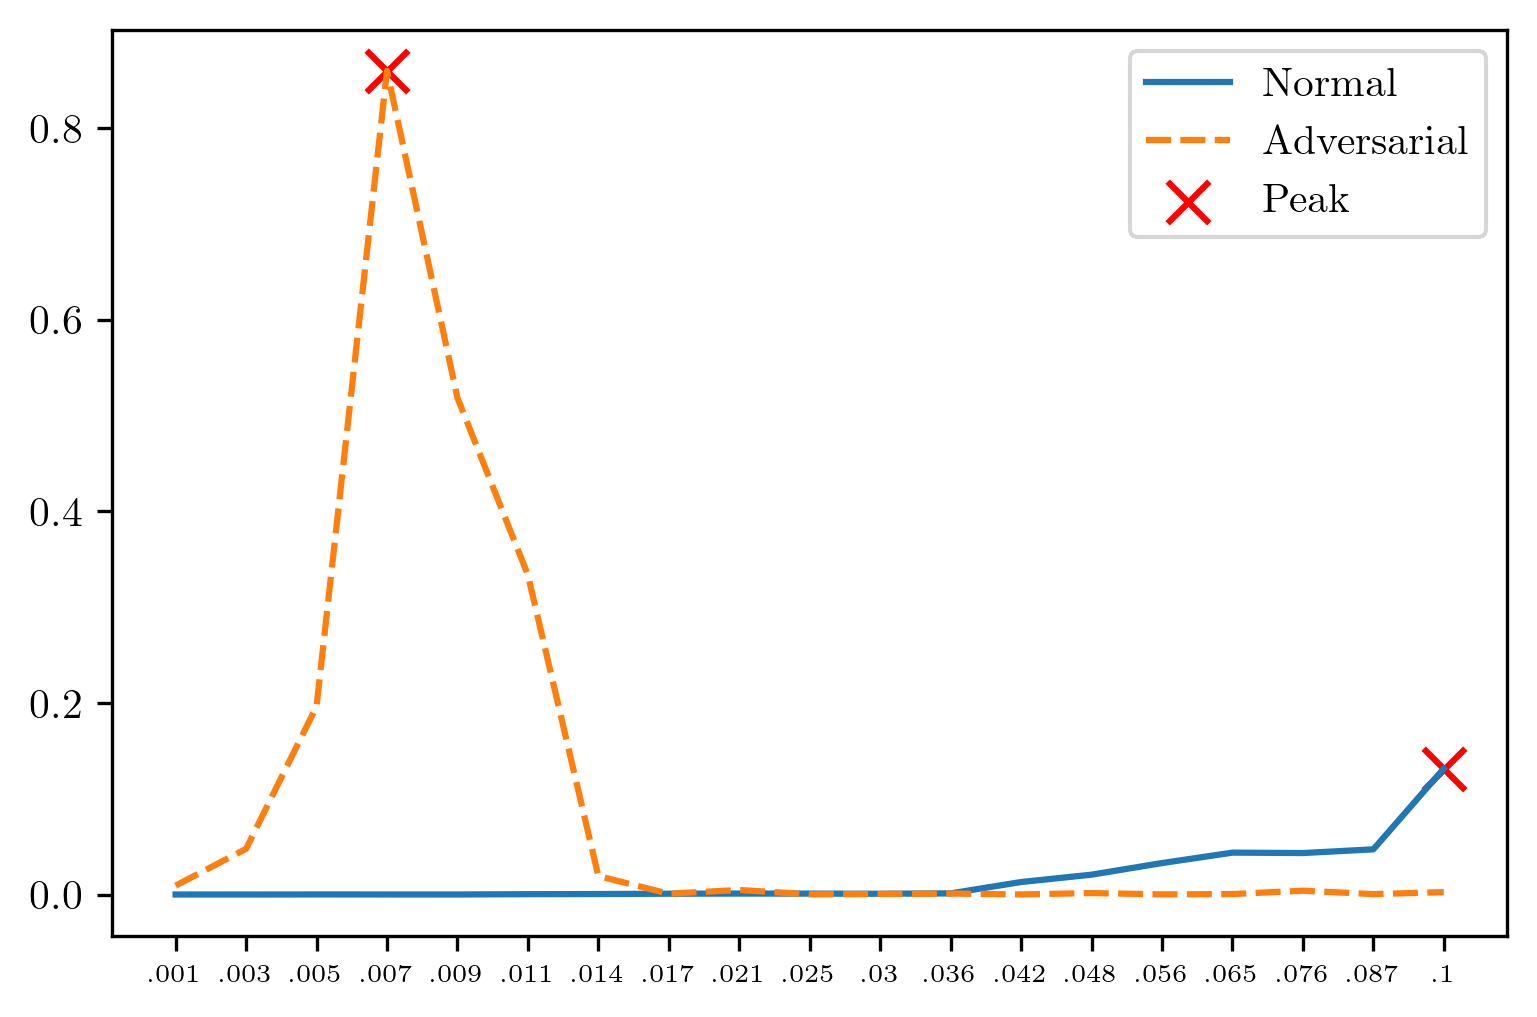
\includegraphics[clip,width=.5\linewidth]{Figures/peaks/1.png}%
    }
    \subfloat[]{%
        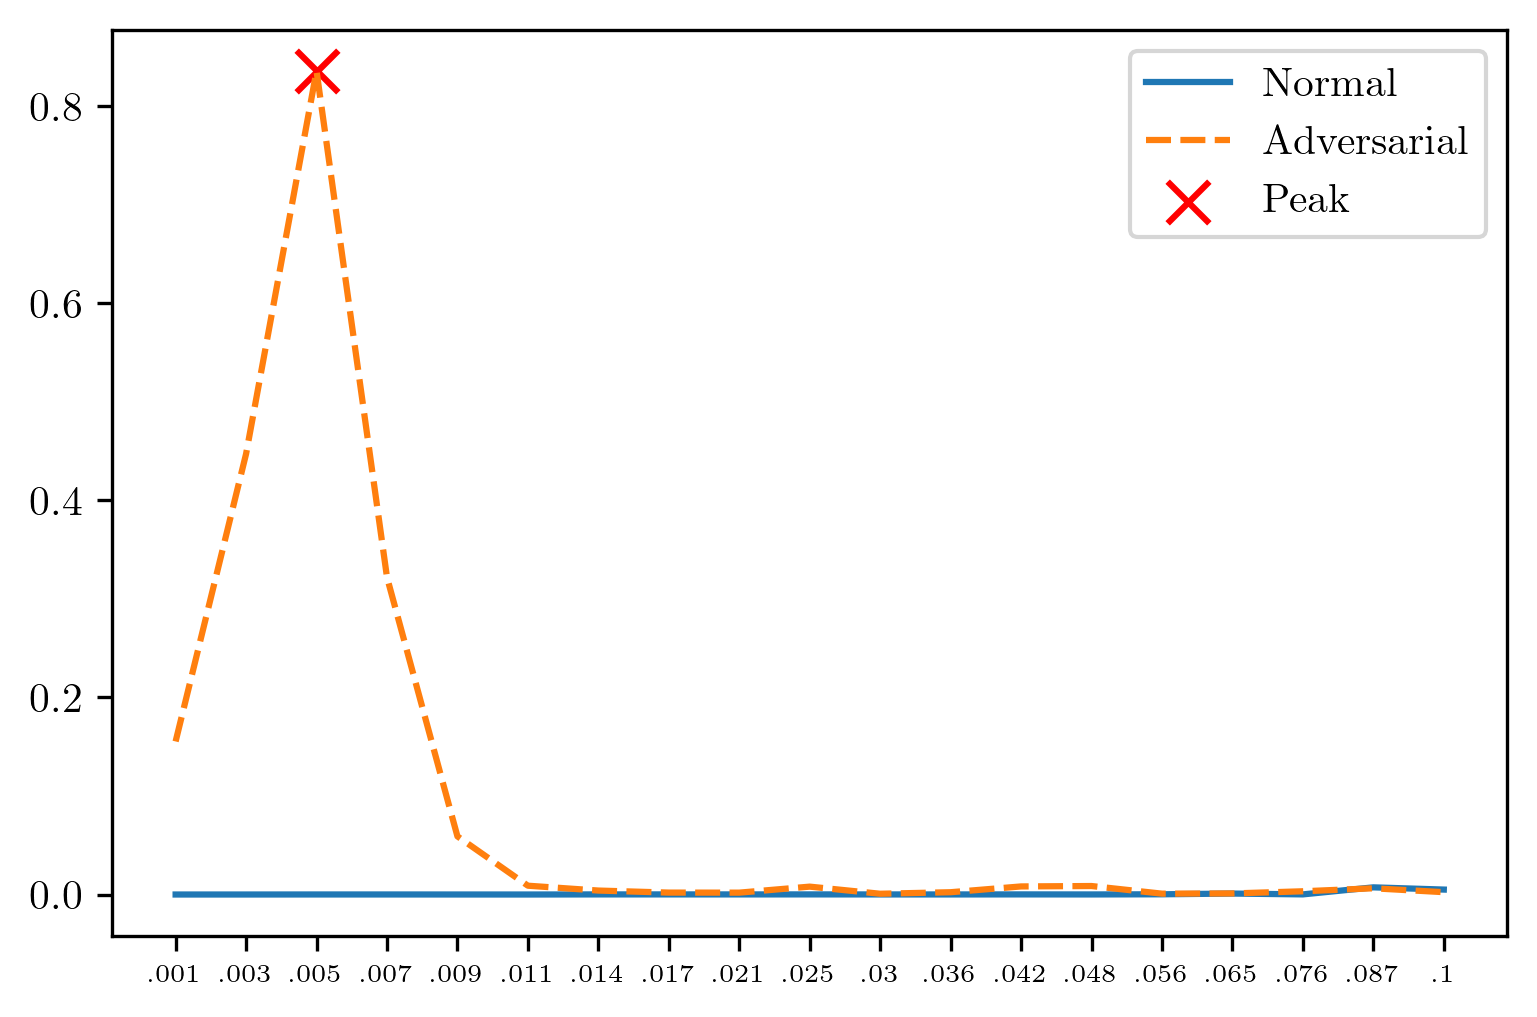
\includegraphics[clip,width=.5\linewidth]{Figures/peaks/3.png}%
    }

    \subfloat[]{%
        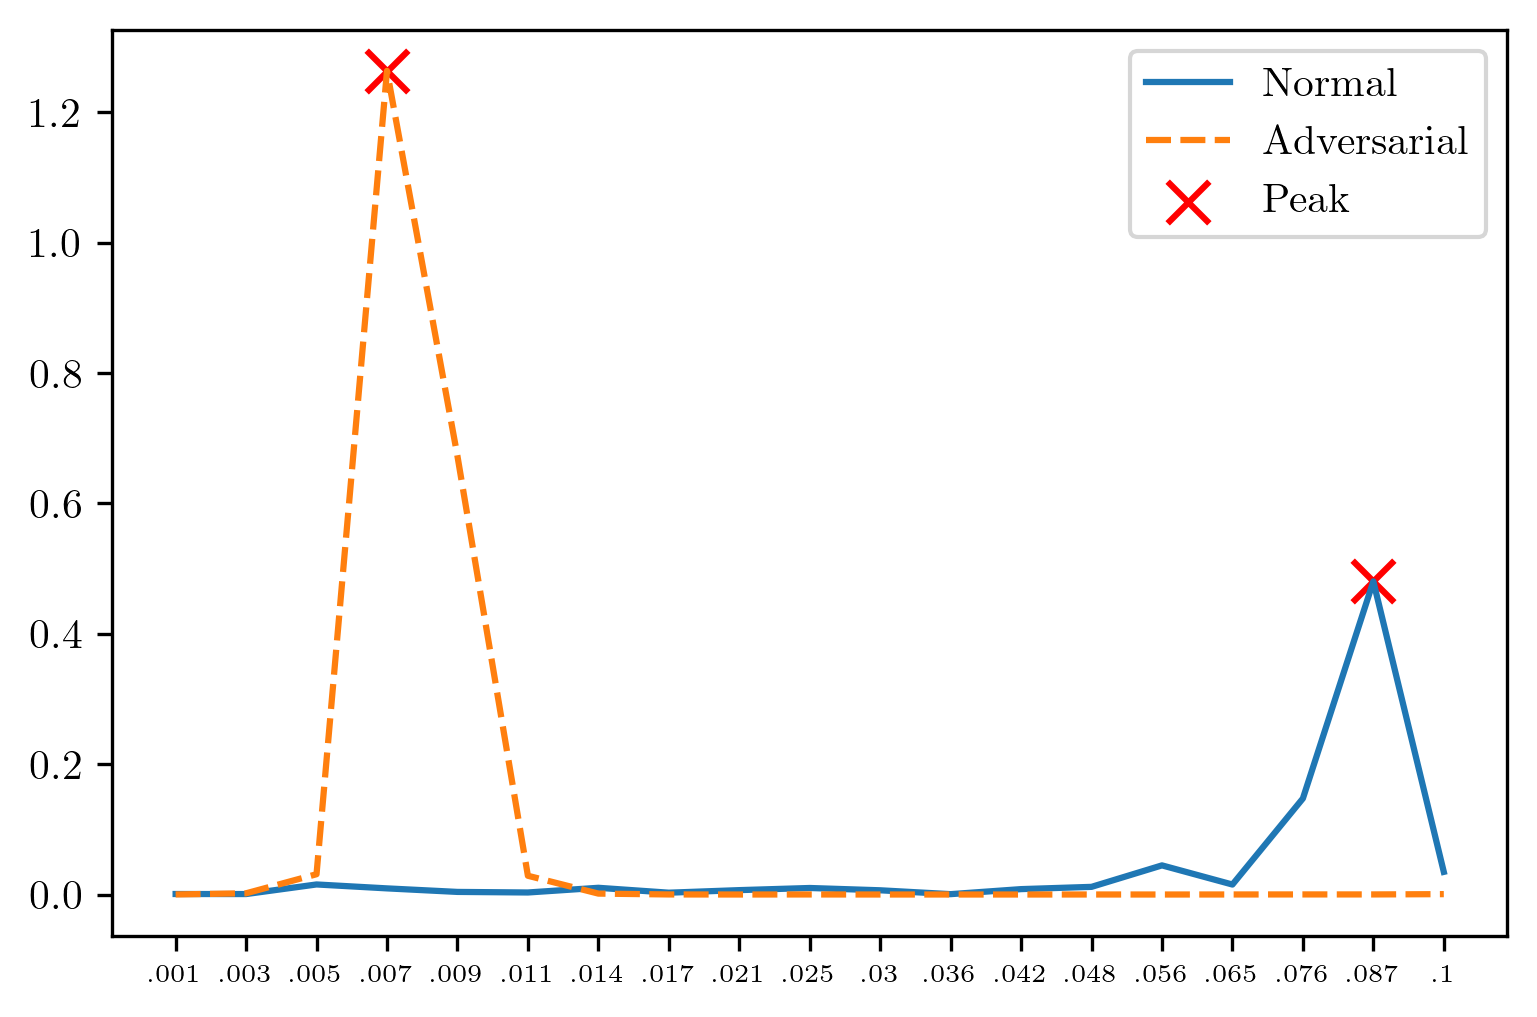
\includegraphics[clip,width=.5\linewidth]{Figures/peaks/13.png}%
    }
    \subfloat[]{%
        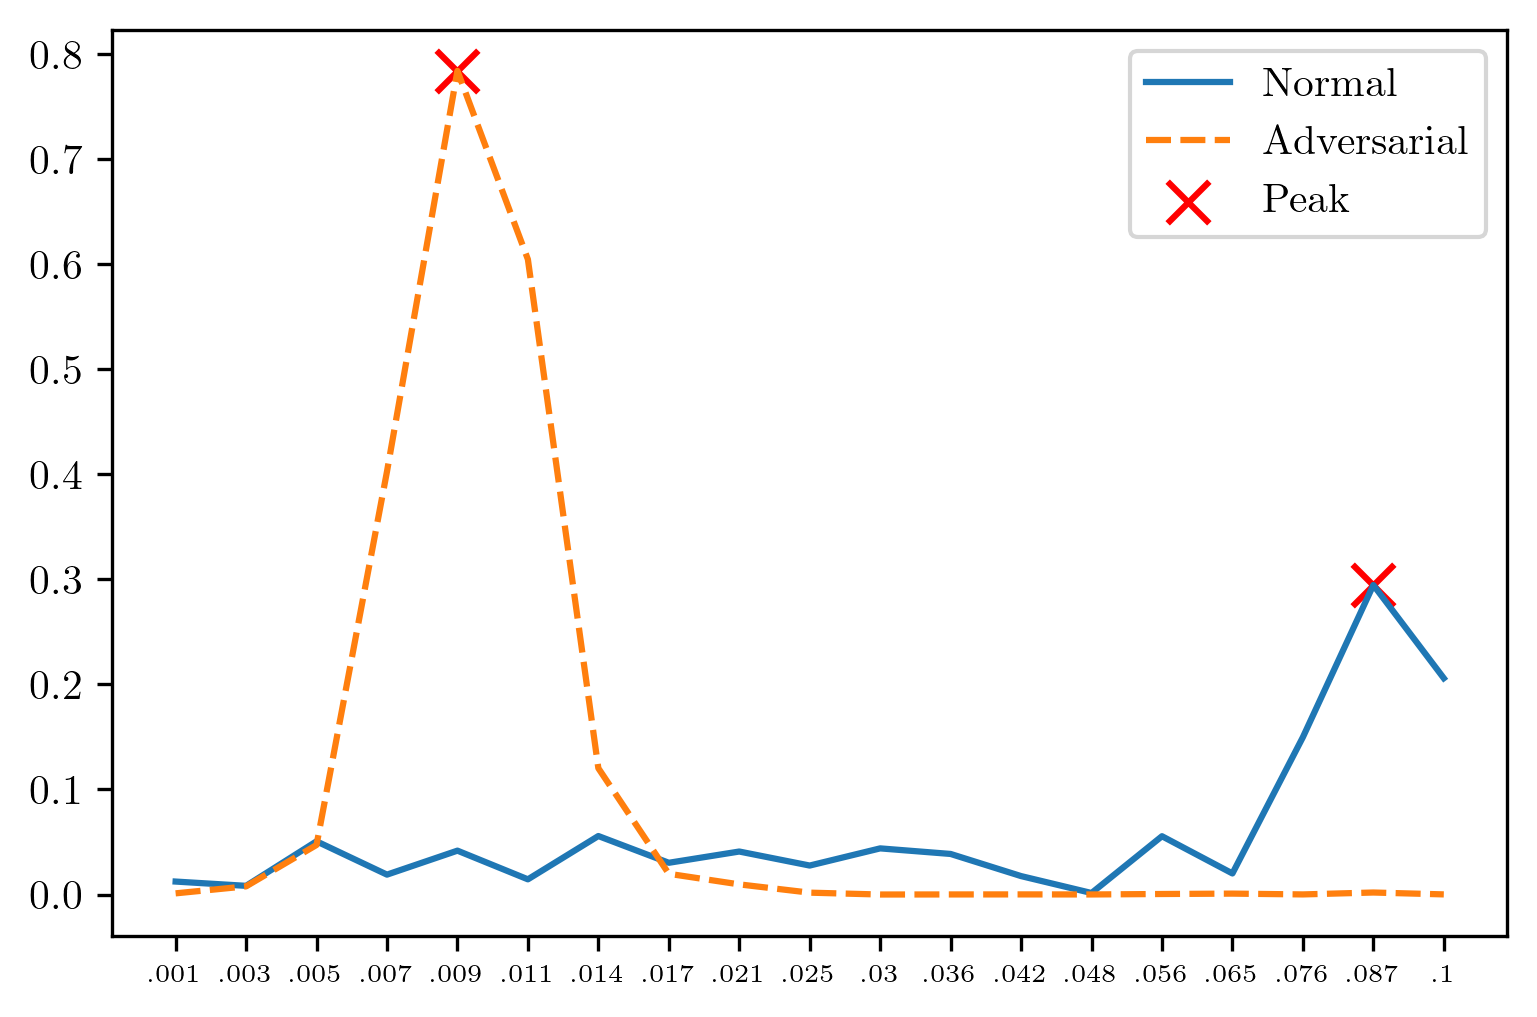
\includegraphics[clip,width=.5\linewidth]{Figures/peaks/20.png}%
    }

    \caption{Peaks observed on normal and adversarial images. Peaks on
        adversarial examples appear to happen at a sooner noise intensity and
        reach a higher value.}
    \label{fig:peaks}
\end{figure}
During my experiments, I wanted to explore different ways of detecting scores
anomalies. One of the ways I briefly experimented with was to plot the scores
differences at each noise intensity step. For example, given ten $\kappa$, I
computed the first-order difference like so:

\begin{align}
    \label{eq:first-order-diff}
    out_i= \lvert \alpha_{i+1} - \alpha_{i} \rvert,
\end{align}
where $\alpha_i$ represents the score result (either $score_1$ or $score_2$ seen
in \ref{eq:score1} and \ref{eq:score2}) at $\kappa_i$ noise intensity.

Figure \ref{fig:peaks} shows the plot of these score differences for four random
images and four adversarial examples generated with different methods. We
observe that the adversarial examples display high peaks earlier than normal
images. In most cases, normal images do not contain peaks at all. This
observation could be used to detect adversarial examples, \emph{e.g.,} by
comparing the intensity of the peaks and when they occur, \emph{i.e.,} when the
first-order difference peaks at an earlier $\kappa$, and at a high magnitude,
this could indicate the adversarial nature of the input.

Furthermore, for future research, I believe the detection performances of my
method could be improved by adding Gaussian noise as a form of data augmentation
during the training phase. Adding noise to the training data has been done
before to reduce overfitting or stabilize the models
\cite{zheng_improving_2016}. However, in combination with my method, I believe
that training the model with randomly modified inputs would improve the model's
robustness to noise and, thus, hypothetically reduce the number of false
positives, especially on lower resolution images like CIFAR-10, which increases
detection precision.